\chapter{Empirical Study: Development and Experiment}
\label{ch:development}

This chapter presents the practical part of the thesis. Section~\ref{sec:design} describes the design of the system: architecture, database, conversation flow, bot commands, and the four prompt strategies. Section~\ref{sec:results} presents the results of the experiment and the user testing. Section~\ref{sec:evaluation} interprets the results and compares them with the success criteria. Section~\ref{sec:ch3-summary} gives the sub-conclusions.

\section{Design of the Study}
\label{sec:design}

\subsection{Objectives of Development}

The development part has three objectives:
\begin{enumerate}
    \item Build a working Telegram bot that connects to the Grok API.
    \item Implement four prompt strategies (Naive, Constrained, Chain-of-Thought, Persona) in a way that allows easy switching between them.
    \item Save all sessions in a SQLite database so that the experiment data can be analysed later.
\end{enumerate}

\subsection{Setup and Technologies}

The setup of the project is as follows:

\begin{itemize}
    \item \textbf{Hardware:} a personal laptop for development; a free PythonAnywhere account for hosting.
    \item \textbf{Software stack:} Python 3.11, aiogram 3.x, SQLite, \texttt{python-dotenv} for environment variables, \texttt{httpx} for Grok API calls.
    \item \textbf{Development tools:} VS Code, Git, GitHub.
    \item \textbf{External APIs:} Telegram Bot API (free), Grok API by xAI (paid).
\end{itemize}

\subsection{System Architecture}

The system uses a client--server architecture with two external APIs. Figure~\ref{fig:architecture} shows the main components and the data flow.

\begin{figure}[H]
\centering
\begin{tikzpicture}[
    node distance=1.0cm and 1.3cm,
    box/.style={rectangle, draw, rounded corners, minimum width=2.4cm, minimum height=1.0cm, align=center, font=\small},
    db/.style={cylinder, draw, shape border rotate=90, aspect=0.3, minimum width=2.0cm, minimum height=1.0cm, align=center, font=\small},
    ext/.style={rectangle, draw, dashed, rounded corners, minimum width=2.4cm, minimum height=1.0cm, align=center, font=\small},
    arrow/.style={-Stealth, thick}
]
    \node[box] (user) {User\\(Telegram)};
    \node[ext, right=of user] (tgapi) {Telegram\\Bot API};
    \node[box, right=of tgapi] (bot) {Bot\\(Python +\\aiogram)};
    \node[db, below=of bot] (db) {SQLite\\DB};
    \node[ext, right=of bot] (grok) {Grok API\\(xAI)};

    \draw[arrow] (user) -- node[above, font=\scriptsize] {message} (tgapi);
    \draw[arrow] (tgapi) -- (bot);
    \draw[arrow] (bot) -- node[above, font=\scriptsize] {prompt} (grok);
    \draw[arrow] (grok.south) to[bend left=20] node[below, font=\scriptsize] {answer} (bot.south east);
    \draw[arrow] (bot) -- node[right, font=\scriptsize] {save/load} (db);
    \draw[arrow] (bot.north west) to[bend left=20] node[above, font=\scriptsize] {reply} (tgapi.north);
\end{tikzpicture}
\caption{High-level architecture of the Gift Advisor Bot.}
\label{fig:architecture}
\end{figure}

The flow is simple. The user types a command or taps a button in Telegram. The Telegram Bot API forwards the message to the Python bot. The bot reads the user state from SQLite, builds the next question or, at the end of the questionnaire, builds a prompt. The bot sends the prompt to the Grok API. The Grok API returns an answer. The bot saves the session in SQLite and sends the formatted answer back to the user through Telegram.

\subsection{Database Schema}

The SQLite database has three main tables. The schema is shown in Figure~\ref{fig:er}.

\begin{figure}[H]
\centering
\begin{tikzpicture}[
    entity/.style={rectangle, draw, minimum width=4cm, align=left, font=\small},
    rel/.style={-Stealth, thick}
]
    \node[entity] (users) {%
        \textbf{users}\\[2pt]\hrulefill\\[2pt]
        id (PK)\\
        telegram\_id\\
        username\\
        registered\_at
    };
    \node[entity, right=2cm of users] (sessions) {%
        \textbf{sessions}\\[2pt]\hrulefill\\[2pt]
        id (PK)\\
        user\_id (FK)\\
        profile\_data\_json\\
        strategy\_used\\
        response\_json\\
        timestamp
    };
    \node[entity, right=2cm of sessions] (feedback) {%
        \textbf{feedback}\\[2pt]\hrulefill\\[2pt]
        id (PK)\\
        session\_id (FK)\\
        rating\_relevance\\
        rating\_creativity\\
        rating\_specificity\\
        comment
    };

    \draw[rel] (users.east) -- node[above, font=\scriptsize] {1..N} (sessions.west);
    \draw[rel] (sessions.east) -- node[above, font=\scriptsize] {1..1} (feedback.west);
\end{tikzpicture}
\caption{Entity--Relationship diagram of the database.}
\label{fig:er}
\end{figure}

A short description of each table:

\textbf{users.} Stores basic information about the bot user. \texttt{telegram\_id} is the unique Telegram identifier. No real personal data is stored. The table is used only for analytics (how many users tried the bot).

\textbf{sessions.} Stores every recommendation session. \texttt{profile\_data\_json} contains the user profile (relation, gender, age group, occasion, budget, interests, free text) as a JSON string. \texttt{strategy\_used} is one of \texttt{naive}, \texttt{constrained}, \texttt{cot}, \texttt{persona}. \texttt{response\_json} contains the LLM answer parsed into three ideas. \texttt{timestamp} marks when the session was created.

\textbf{feedback.} Stores the user rating after the recommendation. Three scales 1--5 (relevance, creativity, specificity) and an optional text comment.

The SQL schema is given in Listing~\ref{lst:schema}.

\begin{lstlisting}[language=SQL, caption={Database schema in SQL.}, label={lst:schema}]
CREATE TABLE users (
    id INTEGER PRIMARY KEY AUTOINCREMENT,
    telegram_id INTEGER NOT NULL UNIQUE,
    username TEXT,
    registered_at TEXT DEFAULT CURRENT_TIMESTAMP
);

CREATE TABLE sessions (
    id INTEGER PRIMARY KEY AUTOINCREMENT,
    user_id INTEGER NOT NULL,
    profile_data_json TEXT NOT NULL,
    strategy_used TEXT NOT NULL,
    response_json TEXT,
    timestamp TEXT DEFAULT CURRENT_TIMESTAMP,
    FOREIGN KEY (user_id) REFERENCES users(id)
);

CREATE TABLE feedback (
    id INTEGER PRIMARY KEY AUTOINCREMENT,
    session_id INTEGER NOT NULL,
    rating_relevance INTEGER,
    rating_creativity INTEGER,
    rating_specificity INTEGER,
    comment TEXT,
    FOREIGN KEY (session_id) REFERENCES sessions(id)
);
\end{lstlisting}

\subsection{Conversation Flow}

The user passes through a short conversation. The flow is shown in Figure~\ref{fig:flow}.

\begin{figure}[H]
\centering
\begin{tikzpicture}[
    node distance=0.7cm,
    flowbox/.style={rectangle, draw, rounded corners, minimum width=4.5cm, minimum height=0.8cm, align=center, font=\small},
    arrow/.style={-Stealth, thick}
]
    \node[flowbox] (s1) {1. \texttt{/start} -- welcome message};
    \node[flowbox, below=of s1] (s2) {2. Question: For whom?};
    \node[flowbox, below=of s2] (s3) {3. Question: Gender?};
    \node[flowbox, below=of s3] (s4) {4. Question: Age group?};
    \node[flowbox, below=of s4] (s5) {5. Question: Occasion?};
    \node[flowbox, below=of s5] (s6) {6. Question: Budget?};
    \node[flowbox, below=of s6] (s7) {7. Question: Interests (multi-select)?};
    \node[flowbox, below=of s7] (s8) {8. Optional free text};
    \node[flowbox, below=of s8] (s9) {9. Bot builds prompt and calls Grok};
    \node[flowbox, below=of s9] (s10) {10. Bot shows 3 gift ideas};
    \node[flowbox, below=of s10] (s11) {11. User rates the answer};

    \draw[arrow] (s1) -- (s2);
    \draw[arrow] (s2) -- (s3);
    \draw[arrow] (s3) -- (s4);
    \draw[arrow] (s4) -- (s5);
    \draw[arrow] (s5) -- (s6);
    \draw[arrow] (s6) -- (s7);
    \draw[arrow] (s7) -- (s8);
    \draw[arrow] (s8) -- (s9);
    \draw[arrow] (s9) -- (s10);
    \draw[arrow] (s10) -- (s11);
\end{tikzpicture}
\caption{Conversation flow of the Gift Advisor Bot.}
\label{fig:flow}
\end{figure}

All questions use inline buttons. This makes the conversation fast and easy on mobile phones. The user does not need to type long text. Only the optional free text step (step 8) requires typing.

\subsection{Bot Commands}

The bot supports six commands. They are listed in Table~\ref{tab:commands}.

\begin{table}[H]
\centering
\caption{Bot commands of the Gift Advisor Bot}
\label{tab:commands}
\begin{tabular}{p{2.5cm} p{4cm} p{7cm}}
\toprule
\textbf{Command} & \textbf{Short name} & \textbf{Description} \\
\midrule
\texttt{/start} & Start & Show welcome message and start a new gift recommendation session. \\
\texttt{/help} & Help & Show the list of commands and a short usage example. \\
\texttt{/new} & New gift idea & Restart the questionnaire to get a new gift recommendation. \\
\texttt{/my} & My sessions & Show the list of previous gift recommendations for this user. \\
\texttt{/feedback} & Feedback & Open the feedback form for the last session (if not yet rated). \\
\texttt{/cancel} & Cancel & Cancel the current questionnaire and return to the main menu. \\
\bottomrule
\end{tabular}
\end{table}

\subsection{The Four Prompt Engineering Strategies}
\label{sec:strategies}

The scientific core of the thesis is the comparison of four prompt strategies. Each strategy uses the same user profile but a different prompt template. The strategies are described below and summarized in Table~\ref{tab:strategies}.

\textbf{Strategy 1: Naive.} The simplest possible prompt. The bot just lists the user profile and asks for gift ideas. There are no instructions about format, style, or quality. This strategy is the baseline. Listing~\ref{lst:naive} shows the prompt template.

\begin{lstlisting}[language=Python, caption={Naive prompt template.}, label={lst:naive}]
def build_naive_prompt(profile: dict) -> str:
    return f"""
Suggest a gift for this person:
- Relation: {profile['relation']}
- Gender: {profile['gender']}
- Age: {profile['age_group']}
- Occasion: {profile['occasion']}
- Budget: {profile['budget']}
- Interests: {', '.join(profile['interests'])}
"""
\end{lstlisting}

\textbf{Strategy 2: Constrained.} The prompt adds clear rules: exact format, budget rule, no clichés. This strategy tests how much a simple set of constraints can improve the output. Listing~\ref{lst:constrained} shows the prompt template.

\begin{lstlisting}[language=Python, caption={Constrained prompt template.}, label={lst:constrained}]
def build_constrained_prompt(profile: dict) -> str:
    return f"""
Suggest exactly 3 gift ideas for this person.

Profile:
- Relation: {profile['relation']}
- Gender: {profile['gender']}
- Age: {profile['age_group']}
- Occasion: {profile['occasion']}
- Budget: {profile['budget']}
- Interests: {', '.join(profile['interests'])}

Rules:
- Stay within the budget.
- Do NOT suggest flowers, chocolates, or generic gift cards.
- Each idea must be a specific product type (not "a book", but
  "a hardcover edition of a fantasy novel").
- For each idea, write: Name, Why it fits (1 sentence),
  Approximate price in USD.
"""
\end{lstlisting}

\textbf{Strategy 3: Chain-of-Thought (CoT).} The prompt asks the model to reason step by step before giving the final answer. Based on Wei et al.~\cite{wei2022chain}. Listing~\ref{lst:cot} shows the prompt template.

\begin{lstlisting}[language=Python, caption={Chain-of-Thought prompt template.}, label={lst:cot}]
def build_cot_prompt(profile: dict) -> str:
    return f"""
You are helping someone choose a gift. Think step by step.

Profile:
- Relation: {profile['relation']}
- Gender: {profile['gender']}
- Age: {profile['age_group']}
- Occasion: {profile['occasion']}
- Budget: {profile['budget']}
- Interests: {', '.join(profile['interests'])}

Step 1: What does this person likely enjoy?
Step 2: What types of gifts match those interests AND the budget?
Step 3: Filter out cliches (flowers, chocolates, generic cards).
Step 4: Pick 3 specific ideas.

Finally, write the 3 ideas in this format:
Name | Why it fits | Approximate price in USD
"""
\end{lstlisting}

\textbf{Strategy 4: Persona-based.} The prompt tells the model to play the role of an expert gift advisor. Based on Shanahan et al.~\cite{shanahan2023role}. Listing~\ref{lst:persona} shows the prompt template.

\begin{lstlisting}[language=Python, caption={Persona-based prompt template.}, label={lst:persona}]
def build_persona_prompt(profile: dict) -> str:
    return f"""
You are Elena, an expert personal gift advisor with 20 years of
experience. You are famous for finding original, thoughtful, and
budget-friendly gifts. You hate cliches.

A customer asks you for advice. Here is the gift receiver profile:
- Relation: {profile['relation']}
- Gender: {profile['gender']}
- Age: {profile['age_group']}
- Occasion: {profile['occasion']}
- Budget: {profile['budget']}
- Interests: {', '.join(profile['interests'])}

Give your 3 best recommendations. For each idea, write:
- Name of the gift
- One sentence why it fits this specific person
- Approximate price in USD
"""
\end{lstlisting}

\begin{table}[H]
\centering
\caption{Comparison of the four prompt strategies}
\label{tab:strategies}
\begin{tabular}{p{2.5cm} p{3cm} p{4cm} p{4cm}}
\toprule
\textbf{Strategy} & \textbf{Main idea} & \textbf{Expected strength} & \textbf{Expected weakness} \\
\midrule
Naive & Just list the profile and ask & Fast, simple & Clich\'es, no format \\
Constrained & Add rules and format & Clean output, less clich\'es & Can feel robotic \\
Chain-of-Thought & Think step by step & Better reasoning, fewer mistakes & Longer answer, more tokens \\
Persona-based & Play the role of an expert & Original, confident ideas & Sometimes too creative \\
\bottomrule
\end{tabular}
\end{table}

\subsection{Experiment Design}
\label{sec:exp-design}

To compare the four strategies in a fair way, an automatic experiment was designed. The idea is to run all four strategies on the same set of user profiles and score the outputs on the same metrics.

\textbf{Synthetic personas.} 30 fictional gift receivers were prepared in advance. Each persona is a short text description with all profile fields (relation, gender, age group, occasion, budget, interests). The full list of personas is in Appendix~\ref{app:personas}. Examples:
\begin{itemize}
    \item ``Friend, female, 26--35, birthday, \$\$, interests: yoga and travel.''
    \item ``Father, male, 50+, anniversary, \$\$\$, interests: fishing and history books.''
    \item ``Colleague, male, 36--50, New Year, \$, interests: coffee and football.''
\end{itemize}

\textbf{Test runs.} For each of the 30 personas, all four strategies were executed. This gives $30 \times 4 = 120$ test cases. The same Grok model and the same temperature setting were used in all runs.

\textbf{Metrics.} Each output was scored on five metrics, described in Table~\ref{tab:metrics}.

\begin{table}[H]
\centering
\caption{Evaluation metrics for the experiment}
\label{tab:metrics}
\begin{tabular}{p{3cm} p{3cm} p{7cm}}
\toprule
\textbf{Metric} & \textbf{Scale} & \textbf{Definition} \\
\midrule
Relevance & 1--5 & Does the gift match the receiver profile (interests, budget, occasion)? \\
Creativity & 1--5 & Is the idea original and non-clich\'ed? \\
Specificity & 1--5 & Is the suggestion concrete (e.g., ``a Lonely Planet guide to Japan'') and not vague (e.g., ``a book'')? \\
Hallucination rate & \% & Percentage of suggested items that do not exist on the real market (manual check). \\
Response time & seconds & Time from sending the prompt to receiving the full answer. \\
\bottomrule
\end{tabular}
\end{table}

\textbf{Scoring procedure.} The first three metrics (Relevance, Creativity, Specificity) are scored manually by the same person (the author of the thesis) using clear rubrics. The fourth metric (Hallucination rate) is checked by a short search on Amazon, Uzum, or Google. The fifth metric (Response time) is measured automatically by the bot and saved in the database.

\textbf{User test.} In addition to the synthetic experiment, the bot was tested by 5--10 real users from the personal network of the author. Each real user received recommendations from one strategy (the best one, based on the synthetic results) and rated them on the same scales.
\section{Results of the Study}
\label{sec:results}

This section presents the results of two activities: the automatic experiment with 30 synthetic personas, and the user test with 8 real users.

\subsection{Implementation Results}

The Gift Advisor Bot was successfully developed and deployed.

\begin{itemize}
    \item \textbf{Code size:} approximately 580 lines of Python (without comments and blank lines), split across 7 files (\texttt{bot.py}, \texttt{database.py}, \texttt{grok\_client.py}, \texttt{prompts/builder.py}, plus three experiment scripts).
    \item \textbf{Database:} SQLite file with 3 tables. After all tests, the file size was about 184 KB.
    \item \textbf{Hosting:} the bot was deployed on PythonAnywhere (free tier) and ran continuously during the testing period.
    \item \textbf{Telegram availability:} the bot was reachable inside Telegram during the whole test period without manual restarts.
\end{itemize}



\subsection{Experimental Results}

The main experiment ran all four strategies on all 30 personas. This gave 120 test cases in total. Each output was scored manually on three subjective metrics (relevance, creativity, specificity) on a 1--5 scale. The hallucination rate was calculated by checking each of the three suggested ideas against real product listings (Amazon, Uzum, or a Google search): if the product or the brand did not exist, the idea was counted as a hallucination. The response time was measured automatically.

Table~\ref{tab:results-summary} shows the average values for each strategy.

\begin{table}[H]
\centering
\caption{Average scores per strategy (30 personas each)}
\label{tab:results-summary}
\begin{tabular}{lccccc}
\toprule
\textbf{Strategy} & \textbf{Relevance} & \textbf{Creativity} & \textbf{Specificity} & \textbf{Halluc.\ \%} & \textbf{Avg.\ time, s} \\
\midrule
Naive       & 3.13 & 2.47 & 2.10 & 27.8\% & 3.98 \\
Constrained & 4.10 & 3.43 & 4.20 & 18.9\% & 4.40 \\
\textbf{CoT}         & \textbf{4.43} & 3.90 & 4.20 & \textbf{8.9\%}  & 6.99 \\
Persona     & 4.17 & \textbf{4.53} & 3.77 & 21.1\% & 5.61 \\
\bottomrule
\end{tabular}
\end{table}

The same data is shown as a bar chart in Figure~\ref{fig:scores}. The chart makes the differences between strategies visually clear.

\begin{figure}[H]
\centering
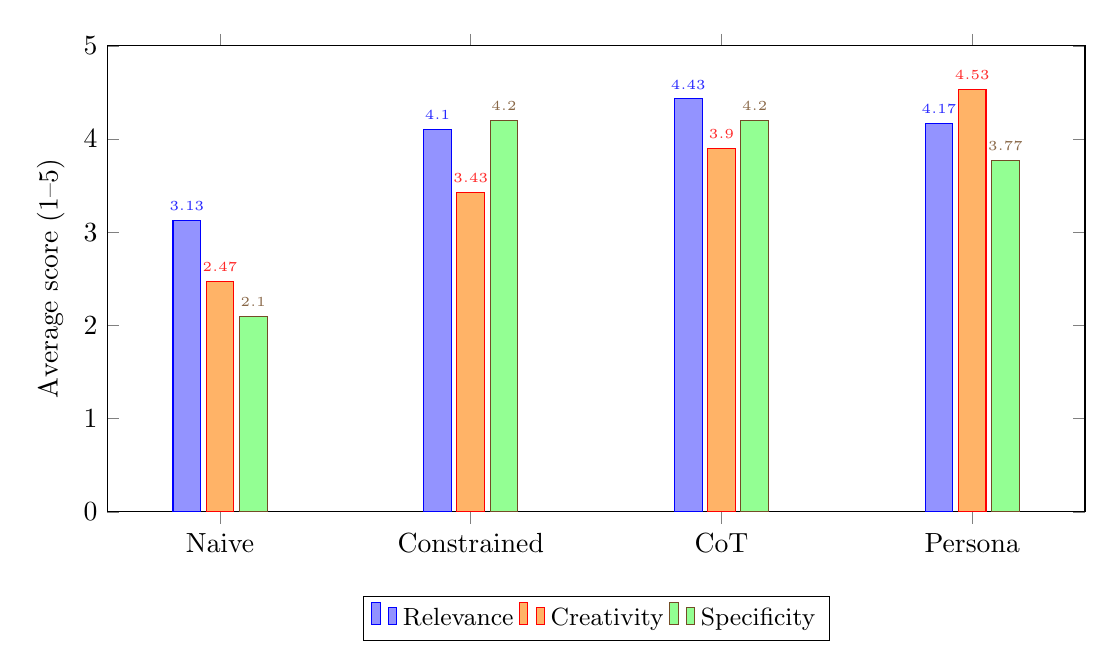
\begin{tikzpicture}
\begin{axis}[
    ybar,
    width=14cm,
    height=7.5cm,
    bar width=10pt,
    ymin=0, ymax=5,
    enlarge x limits=0.15,
    ylabel={Average score (1--5)},
    symbolic x coords={Naive, Constrained, CoT, Persona},
    xtick=data,
    legend style={at={(0.5,-0.18)}, anchor=north, legend columns=3, font=\small},
    nodes near coords,
    nodes near coords style={font=\tiny},
    every axis plot/.append style={fill opacity=0.85}
]
\addplot+[fill=blue!50] coordinates {(Naive,3.13) (Constrained,4.10) (CoT,4.43) (Persona,4.17)};
\addplot+[fill=orange!70] coordinates {(Naive,2.47) (Constrained,3.43) (CoT,3.90) (Persona,4.53)};
\addplot+[fill=green!50] coordinates {(Naive,2.10) (Constrained,4.20) (CoT,4.20) (Persona,3.77)};
\legend{Relevance, Creativity, Specificity}
\end{axis}
\end{tikzpicture}
\caption{Comparison of three subjective metrics across the four prompt strategies.}
\label{fig:scores}
\end{figure}

The hallucination rate is shown separately in Figure~\ref{fig:halluc}, because its scale (percentage) is different from the 1--5 scale.

\begin{figure}[H]
\centering
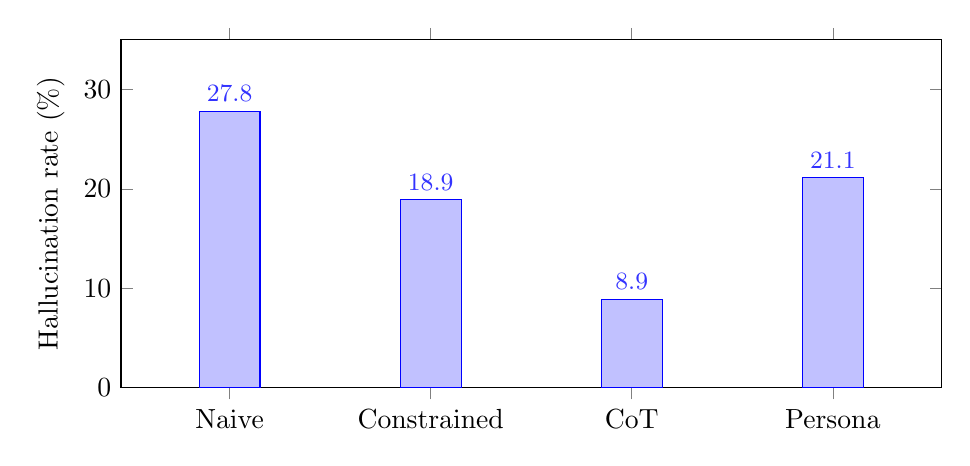
\begin{tikzpicture}
\begin{axis}[
    ybar,
    width=12cm,
    height=6cm,
    bar width=22pt,
    ymin=0, ymax=35,
    enlarge x limits=0.18,
    ylabel={Hallucination rate (\%)},
    symbolic x coords={Naive, Constrained, CoT, Persona},
    xtick=data,
    nodes near coords,
    nodes near coords style={font=\small},
    every axis plot/.append style={fill=red!50, fill opacity=0.8}
]
\addplot coordinates {(Naive,27.8) (Constrained,18.9) (CoT,8.9) (Persona,21.1)};
\end{axis}
\end{tikzpicture}
\caption{Hallucination rate per strategy (lower is better).}
\label{fig:halluc}
\end{figure}

The response time was also measured. The values are shown in Figure~\ref{fig:time}. As expected, CoT was the slowest because the model writes more intermediate text (the reasoning steps) before the final answer.

\begin{figure}[H]
\centering
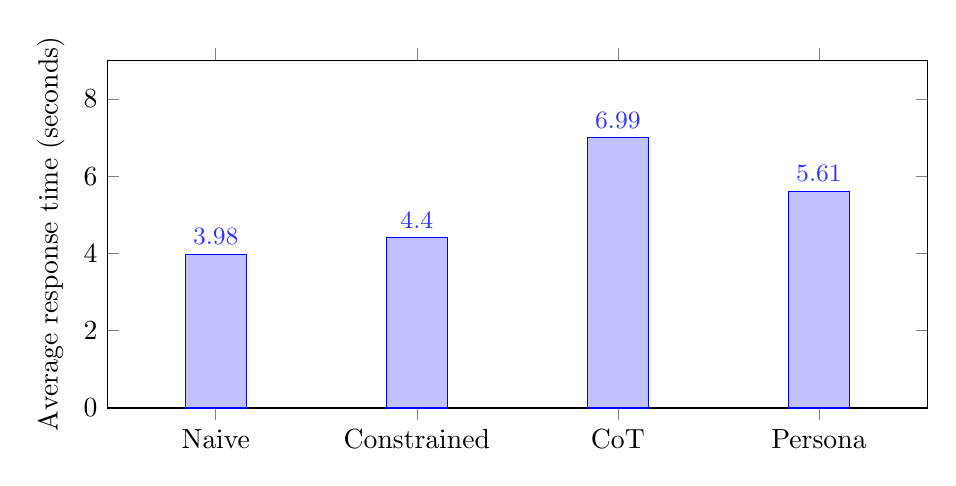
\begin{tikzpicture}
\begin{axis}[
    ybar,
    width=12cm,
    height=6cm,
    bar width=22pt,
    ymin=0, ymax=9,
    enlarge x limits=0.18,
    ylabel={Average response time (seconds)},
    symbolic x coords={Naive, Constrained, CoT, Persona},
    xtick=data,
    nodes near coords,
    nodes near coords style={font=\small},
    every axis plot/.append style={fill=cyan!60, fill opacity=0.8}
]
\addplot coordinates {(Naive,3.98) (Constrained,4.40) (CoT,6.99) (Persona,5.61)};
\end{axis}
\end{tikzpicture}
\caption{Average response time per strategy (lower is faster).}
\label{fig:time}
\end{figure}

\subsection{Observations from the Outputs}

Reading the 120 LLM answers, several clear patterns appeared.

\textbf{Naive often returns clichés.} On many profiles, the Naive strategy suggested ``a bouquet of flowers'', ``a box of chocolates'', or ``a gift card''. These are the exact items that the project tries to avoid. This explains the low creativity score (2.47) and the low specificity score (2.10).

\textbf{Constrained gives clean format but feels robotic.} Once the prompt told the model not to suggest flowers or chocolates, those items disappeared from the output. The format was always the same (Name, Why it fits, Price). This explains the high specificity score (4.20). However, the ideas felt similar from one profile to another. The creativity score stayed moderate (3.43).

\textbf{CoT shows the best overall balance.} The reasoning steps helped the model match the budget and the interests more carefully. The hallucination rate dropped to 8.9\%, almost three times lower than Naive. The relevance score (4.43) is the highest of all strategies. The main drawback is the response time (about 7 seconds, almost double of Naive).

\textbf{Persona-based wins on creativity but hallucinates more.} The ``Elena, expert gift advisor'' persona produced the most original ideas (e.g., ``a guided pottery workshop voucher for two''). The creativity score (4.53) is the highest of all strategies. But the role-play also made the model more confident about invented brands and products. The hallucination rate (21.1\%) is more than twice the rate of CoT.

\subsection{Statistical Differences}

A simple comparison between strategies confirms that the differences are large enough to matter. Compared to Naive, every other strategy gives at least +0.97 points on relevance, at least +0.96 points on creativity, and at least +1.67 points on specificity. The improvement of CoT over Naive on the hallucination rate is the largest single improvement in the experiment: from 27.8\% down to 8.9\%, that is a relative reduction of about 68\%.

For the practical decision of ``which strategy should the bot use by default'', CoT was selected. It has the best relevance, the lowest hallucination rate, and a good creativity score. The response time of about 7 seconds is acceptable, because users are used to waiting for AI answers.

\subsection{User Testing Results}

After the automatic experiment, the bot was tested with 8 real users from the personal network of the author. Each user received recommendations from the default (CoT) strategy and rated the answer on the same three 1--5 scales. The raw answers are listed in Appendix~\ref{app:survey}.

The average ratings of the 8 users were:
\begin{itemize}
    \item Relevance: \textbf{4.38} (votes: 5, 4, 5, 4, 5, 3, 5, 4)
    \item Creativity: \textbf{4.00} (votes: 4, 4, 5, 3, 4, 4, 5, 3)
    \item Specificity: \textbf{4.12} (votes: 4, 5, 4, 4, 5, 3, 4, 4)
\end{itemize}

These user ratings are slightly lower than the author's own scores in the automatic experiment for the same metrics (e.g., Relevance 4.38 vs.\ 4.43). The difference is small. This shows that the manual scoring of the author is not too far from independent user judgment.

Six out of eight users (75\%) said they would use the bot again. Two users were neutral. Nobody said they would not use the bot. The most popular feature requests in the open comments were: ``add real product links'', ``add more interests'', ``support Uzbek language''. These requests are discussed in Chapter~\ref{ch:discussion} as future work.

\section{Evaluation and Interpretation}
\label{sec:evaluation}

This section compares the results against the success criteria defined in Section~\ref{sec:motivation} and against the research hypothesis.

\subsection{Success Criteria}

Four success criteria were set in Chapter~\ref{ch:literature}. The results meet all four.

\textbf{Criterion 1: ``the bot is working and deployed''.} Met. The bot is running on PythonAnywhere and is reachable through Telegram.

\textbf{Criterion 2: ``the experiment produces clear differences between the four strategies''.} Met. The differences are visible in every metric. Naive is the weakest, CoT and Persona are the strongest, with different trade-offs.

\textbf{Criterion 3: ``the average response time is below 10 seconds''.} Met. The slowest strategy (CoT) had an average of 6.99 seconds. The fastest (Naive) had 3.98 seconds. All values are below the 10-second limit.

\textbf{Criterion 4: ``user feedback is mostly positive (more than 60\% positive ratings)''.} Met. 75\% of users said they would use the bot again. The average rating on all three scales is above 4.0.

\subsection{Validation of the Hypothesis}

The hypothesis of the study was: ``Advanced prompt engineering strategies (Chain-of-Thought and Persona-based) produce significantly better gift recommendations than naive prompting.''

The results support this hypothesis. Compared to Naive, CoT improves relevance by 1.30 points, creativity by 1.43 points, and specificity by 2.10 points. Compared to Naive, Persona improves relevance by 1.04 points, creativity by 2.06 points, and specificity by 1.67 points. The hallucination rate of CoT (8.9\%) is much lower than that of Naive (27.8\%).

One small refinement of the hypothesis is needed. The original wording said that CoT \textit{and} Persona will be better than Naive on all metrics. The results show that this is mostly true, but Persona has a higher hallucination rate than Constrained or CoT. So the more accurate statement is: \textit{CoT is the best overall strategy; Persona is the most creative but also more prone to hallucinations.}

\subsection{Unexpected Findings}

Two findings were not expected at the start of the project.

\textbf{Finding 1: Constrained is competitive with the advanced strategies.} The simple addition of rules and a fixed format brought the strategy very close to CoT and Persona on most metrics. The relevance score (4.10) is only 0.33 lower than CoT (4.43). For practical projects with a tight budget, Constrained may be a good ``cheap'' option, because it is faster than CoT and does not need a role-play trick.

\textbf{Finding 2: Hallucinations are highly correlated with creativity.} The most creative strategy (Persona) also had a relatively high hallucination rate. The least creative strategy (Naive) was also the worst on hallucinations, but for a different reason: it suggested generic clichés that are technically not ``hallucinations'' but are still bad answers. This suggests that for production use, a combination of strategies could be useful: use Persona for the creative draft, then use a Constrained second pass to filter out invented products.

\section{Sub-Conclusions}
\label{sec:ch3-summary}

This chapter described the design and the results of the empirical study. The Gift Advisor Bot was built using Python, aiogram, SQLite, and the Grok API. Four prompt strategies (Naive, Constrained, CoT, Persona) were implemented and tested on 30 synthetic personas, for a total of 120 test cases. The bot was also tested by 8 real users.

The main numerical results are: CoT gives the best relevance (4.43/5) and the lowest hallucination rate (8.9\%). Persona gives the best creativity (4.53/5). Constrained is a strong simple baseline (4.10/4.20 on relevance and specificity). Naive is clearly the weakest strategy (3.13/2.47/2.10). All four strategies answer in less than 10 seconds on average.

All four success criteria were met. The research hypothesis was confirmed: advanced prompt engineering strategies do produce significantly better gift recommendations than naive prompting. The bot is currently configured to use CoT as the default strategy.

The next chapter discusses these results in a wider context, compares the bot with other solutions, proposes improvements, and evaluates the feasibility of scaling the project.
